\subsection{Serviceorientierte Architektur}
Eine eindeutige und einheitliche Definition einer Serviceorientierter Architektur (\gls{SOA}) existiert nicht.
Einen Versuch einer Definition wird in \cite{SOA07} beschrieben:
\begin{quote}"`[...] a service oriented
architecture is an architecture for building business applications as a set of
loosely coupled black-box components orchestrated to deliver a well-defined
level of service by linking together business processes."' \begin{flushright}\cite{SOA07} S. 27\end{flushright}\end{quote}
\gls{SOA} ist ein Ansatz im Bereich der Informationstechnik um Anwendungen oder einzelne Dienste aus verschiedenen Geschäftsprozessen zu bilden.\\


Melzer bietet eine ausführlichere Definition:
\begin{quote}"`Unter einer \gls{SOA} versteht man eine Systemarchitektur, die vielfältige, verschiedene und eventuell inkompatible Methoden oder Applikationen als wiederverwendbare und offen zugreifbare Dienste repräsentiert und dadurch eine plattform- und sprachenunabhängige Nutzung und Wiederverwendung ermöglicht.
"' \begin{flushright}\cite{Melzer08} S. 13\end{flushright}\end{quote}
   %\newpage                                              
Zur Verdeutlichung einer \gls{SOA} kann ein beispielhafter und vereinfachter Aufbau eines Online-Shops verwendet werden.

\begin{figure}[ht]
	\centering
	   \fbox{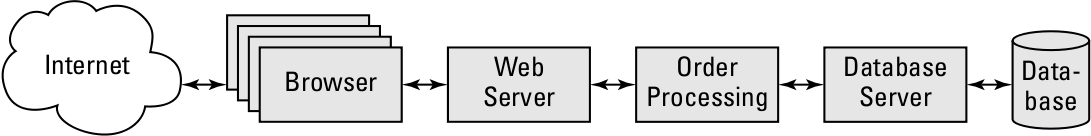
\includegraphics[width=0.9\textwidth]{bilder/soa1.png}}
		\caption[Simple Software Architektur eines Webshops]{Simple Software Architektur eines Webshops\protect\footnote}
		\label{soa1}
\end{figure}
\footnotetext{Quelle: \cite{SOA07} S. 18}

Durch den gewöhnlichen Browser können Benutzer auf die Webseite des Webservers zugreifen um dort auf die eigentliche Anwendung des Webshops \textit{Order Processing} zuzugreifen.
Dabei werden durch einen Datenbankserver die Informationen in einer Datenbank gespeichert oder von dort der Webshop-Anwendung zugänglich gemacht.
Welche Funktion die Anwendung \textit{Order Processing} ausführt hängt von den Aufforderungen des Benutzers durch den Browser ab.
%\newpage
Dieser Struktur wird nun ein Serviceorientierte Komponente \textit{Credit Checking} hinzugefügt, siehe Abbildung \ref{soa2}.

\begin{figure}[ht]
	\centering
	   \fbox{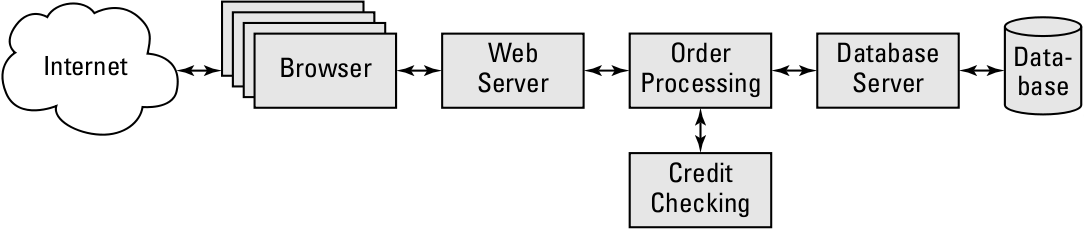
\includegraphics[width=0.85\textwidth]{bilder/soa2.png}}
		\caption[Hinzugefügte Serviceorientierte Komponente]{Hinzugefügte Serviceorientierte Komponente\protect\footnote}
		\label{soa2}
\end{figure}
\footnotetext{Quelle: \cite{SOA07} S. 20}

Dabei hat die eigentliche Anwendung des Webshops keine Kenntnis wie die Komponente \textit{Credit Checking} intern abläuft, sondern übergibt nur die essentiellen Informationen, in diesem Fall die Kreditkartendaten, an die Komponente.
Für die Anwendung ist irrelevant, ob diese Komponenten eine externe Datenbank oder Webseite nach der Kreditwürdigkeit des Benutzers befragen, solange die Komponente auswertbare Informationen (zahlungsfähig ja/nein) an die Webshop-Anwendung liefert.
Für die Anwendung \textit{Order Processing} ist die Komponente \textit{Credit Checking} eine so genannte \textbf{black box}.

Die komplexen Berechnungen und Algorithmen zur Bestimmung der Kreditwürdigkeit des Benutzers werden komplett verdeckt, so dass nur die Kreditkarteninformationen der Komponente zu übergeben sind.

Die Komponente \textit{Credit Checking} steht der Webshop Anwendung als \textbf{abstrahierter Dienst bzw. Service} zur Verfügung.

\subsection{Web-Services-Architektur}
\label{webservice}
Wie bei dem Begriff \gls{SOA} gibt es für Web Services keine allgemein gültige Definition, jedoch überlappen sich Definitionsvorschläge in verschiedenen Gesichtspunkten.
Laut Melzer (\cite{Melzer08} S. 55) bietet das World Wide Web Consortium (\gls{W3C}) den konkretesten Ansatz einer passenden Definition.

\begin{quote}"`A Web service is a software system designed to support interoperable machine-to-machine interaction over a network. It has an interface described in a machine-processable format (specifically \gls{WSDL}). Other systems interact with the Web service in a manner prescribed by its description using \gls{SOAP} messages, typically conveyed using \gls{HTTP} with an \gls{XML} serialization in conjunction with other Web-related standards."' \begin{flushright}\cite{W3WS04} S. 7\end{flushright}\end{quote}

Ein Web Service ist so aufgebaut, dass ein Zusammenspiel zwischen Rechner über ein Netzwerk möglich ist.
Dabei ist Schnittstelle des Web Services in einem maschinell interpretierbaren Format gehalten, so dass andere Systeme auf diese Schnittstelle zugreifen können.
Dieser Zugriff findet durch das Simple Object Access Protocol (\gls{SOAP}) statt, welches üblicherweise über das Hypertext Transfer Protocol (\gls{HTTP}) versendet wird.
Die \gls{SOAP}-Nachrichten sind nach dem \gls{XML}-Schema zusammen mit anderen Web-Standards aufgebaut.
Dadurch können die Nachrichten von beiden Seiten (Client und Server) interpretiert werden.

%This layer is responsible for encoding messages in a common XML format so that messages can be understood at either end. Currently, this includes XML-RPC and SOAP. For example, the client program bundles up two values (see Figure 1) to be added into a SOAP message, which is sent to the Web service by sending it as the body of an HTTP POST request. The server unpacks the SOAP request that the application can understand and executes Add operation. Next, the server packages up that result of summation as response into another SOAP message, which it sends back to the client program in response to its HTTP request. The client program unpacks the SOAP message to obtain the results of the summation. So, SOAP=XML + HTTP. 


Als Beispiel für eine \gls{SOAP}-Kommunikation verschickt ein Client zwei Zahlenwerte, die vom Server addiert werden sollen:
\begin{figure}[ht]
	\centering
	   \fbox{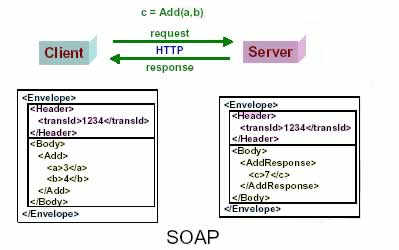
\includegraphics[width=0.85\textwidth]{bilder/nusoap.png}}
	  
		\caption[Kommunikationprotokoll SOAP]{Kommunikationprotokoll SOAP\protect\footnote}
		\label{soa-3eck}
\end{figure}
\footnotetext{\url{http://www.devarticles.com/c/a/PHP/Building-XML-Web-Services-with-PHP-NuSOAP/1/}}

Der Server entpackt die \gls{SOAP}-Nachricht und führt mit den zwei Zahlenwerte die Addition aus.
Das Ergebnis der Rechnung wird im Anschluss wieder als Nachricht im \gls{SOAP}-Format an den Client zurückgesendet.
\newpage
Daraus leitet Melzer folgende Spezifikationen für eine Web-Services-Architektur ab:
\paragraph{SOAP}
beschreibt das \gls{XML}-basierte Nachrichtenformat der Kommunikation und dessen Einbettung in ein Transportprotokoll.
\paragraph{WSDL}
ist eine - ebenfalls \gls{XML}-basierte - Beschreibungssprache, um Web Services (Dienste) zu beschreiben.
\paragraph{UDDI}
beschreibt einen Verzeichnisdienst für Web Services. \gls{UDDI} (Universal Description, Discovery and Integration protocol) spezifiziert eine standardisierte Verzeichnisstruktur für die Verwaltung von Web-Services-Metadaten.
Zu den Metadaten zählen allgemeine Anforderungen, Web-Services-Eigenschaften oder die benötigten Informationen zum Auffinden von Web Services.
\begin{flushright}\cite{Melzer08} S. 55\end{flushright}

Dabei erwähnt Metzer (\cite{Melzer08} S. 56), dass ein Verzeichnisdienst keine Notwendigkeit für die Verwendung eines Web Services ist, "`sondern vielmehr die Infrastruktur zum Auffinden von geeigneten Web Services beschreibt."'


Der Ablauf der Benutzung eines Web Services soll durch Abbildung \ref{soa-3eck} verdeutlicht werden.

\begin{enumerate}
\item Der Anbieter des Web Services muss seinen Dienst durch eine \gls{WSDL}-Datei in Form einer \gls{XML}-Datei dem Dienstverzeichnis bekannt geben.
\item Erst dann können mögliche Nutzer dieses Dienstes den Web Service im \gls{UDDI}-basiertem Dienstverzeichnis finden. Die Suchanfrage findet über eine \gls{SOAP}-Schnittstelle statt.
\item Ein Verweis auf den Dienst in Form einer \gls{WSDL}-Datei wird an den Dienstbenutzer als Antwort der Suchanfrage gesendet.
\item Durch diesen Verweis erfährt der Benutzer die Adresse des Dienstanbieters und kann die Beschreibung des Web Services abfragen.
\item Nach Erhalt dieser Beschreibung kann der eigentliche Webdienst mittels \gls{SOAP} verwendet werden.
\end{enumerate}

\begin{figure}[ht]
	\centering
	   \fbox{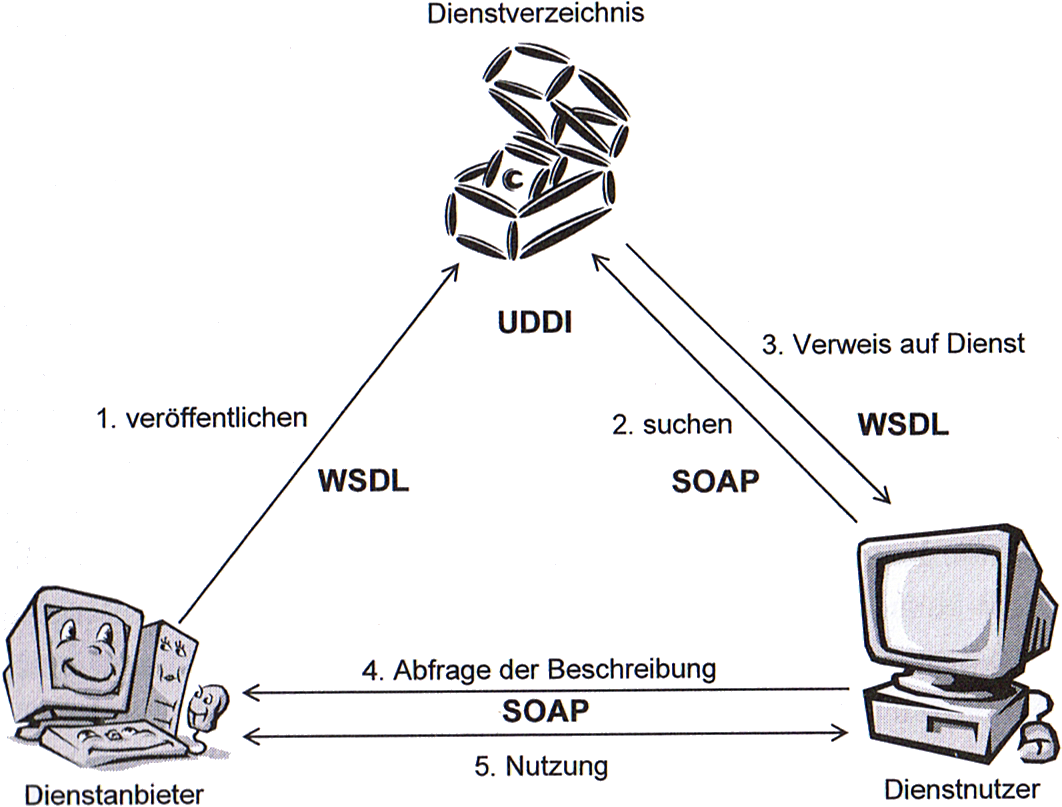
\includegraphics[width=0.85\textwidth]{bilder/uddi-wsdl.png}}
	  
		\caption[Ablauf einer Web Service-Benutzung]{Ablauf einer Web Service-Benutzung\protect\footnote}
		\label{soa-3eck}
\end{figure}
\footnotetext{Quelle: \cite{Melzer08} S. 56}






















